
\documentclass[11pt]{article}
\usepackage[hmargin=1.5cm,vmargin=1.5cm]{geometry}

\usepackage[affil-it]{authblk}
\usepackage[percent]{overpic}

%\usepackage{ifpdf}
%\ifpdf 
%    \usepackage[pdftex]{graphicx}   % to include graphics
%    \pdfcompresslevel=9 
%    \usepackage[pdftex,     % sets up hyperref to use pdftex driver
%            plainpages=false,   % allows page i and 1 to exist in the same document
%            breaklinks=true,    % link texts can be broken at the end of line
%            colorlinks=true,
%            pdftitle=My Document
%            pdfauthor=My Good Self
%           ]{hyperref} 
%    \usepackage{thumbpdf}
%\else 
%    \usepackage{graphicx}       % to include graphics
%    \usepackage{hyperref}       % to simplify the use of \href
%\fi 

\title{Fast Timing Sexy Title}

\author[1]{D.~Anderson, A.~Apresyan, A.~Bornheim, J.~Duarte, C.~Pena, M.~Spiropulu, S.~Xie}
\author[2]{A.~Ronzhin}
\affil[1]{California Institute of Technology, Pasadena, CA, USA}
\affil[2]{Fermi National Accelerator Laboratory, Batavia, USA}

\date{}

\begin{document}

\maketitle
\abstract{Current and future high energy physics particle colliders are capable
to provide instantaneous luminosities of 10$^{34}$ cm$^{-2}$s$^{-1}$ and above.
The high center of mass energy, large number of simultaneous collision of beam
particles in the experiments and the very high repetition rates of the collision
events pose huge challenges. They result in extremely high particle fluxes,
causing very high occupancies in the particle physics detectors operating at
these machines. We discuss how timing information with a precision of around 10
ps and below can aid the reconstruction of the physics events under such
challenging conditions. 

We present studies and measurements from test beams and GEANT4 simulations for
calorimeter based timing measurements to explore the ultimate timing precision
achievable for high-energy photons. We put particular focus on techniques to
measure the timing with a precision of about 10 ps in association with the
energy of the photon. We present studies with detector prototypes where we
achieve the timing resolution of a few tens of picoseconds in test beam
measurements. Finally, possible applications of precision timing in
future high-energy physics experiments are discussed. }



\section{Introduction}
%shorten the LHC discussion to 1 paragraph
%put the TOF cartoon diagram here and discuss the various aspects affects TOF resolution
% say that we have studied 1,4,5 already, and now we focus on 2 and 3 to complete the story.
% briefly introduce the experiments that we did to understand 2 and 3 ( sampling calo with LYSO cube, shashlik with fibers, shashlik with side readout)

Current and future high energy physics particle colliders are capable to provide
instantaneous luminosities of 10$^{34}$ cm$^{-2}$s$^{-1}$ and above. The high
centre of mass energy, the large number of simultaneous collision of beam
particles in the experiments and the very high repetition rates of the collision
events pose huge challenges. They result in extremely high particle fluxes,
causing very high occupancies in the particle physics detectors operating at
these machines. To reconstruct the physics events, the detectors have to make as
much information as possible available on the final state particles. In addition to
the detailed spatial information of the final state particles, as well as their
momenta and energies, one can make use of the relative time of arrival at a given
location in the detector. The work presented in this document is targeted to
address the challenges posed by the experimental conditions expected for the
high luminosity upgrade of the Large Hadron Collider (HL-LHC) at CERN. 

During the HL-LHC operations the expected instantaneous luminosity is estimated
to be $\mathcal{L}\geq$10$^{34}$~cm$^{-2}$s$^{-1}$, resulting in 140 to 200
simultaneous proton-proton collisions that occur every 25 nsec. The luminous
region inside the detector (the location where the protons collide) will have a
length of a few 10 cm. Due to the size of the proton bunches and the resulting
time it takes for them to pass through each other in the luminous region, the
collisions are spread out in time. During the 2011-2012 operation of LHC this
spread was about 200 ps. For HL-LHC this spread may increase as a consequence of
an advanced beam optics of the interaction region. 

The ATLAS and CMS detectors at the LHC are expected to undergo significant
upgrades and modifications, although the basic geometric layout and size will
remain unchanged. In this work we assume that a detector capable of measuring
the time of arrival of a particle would be located at the outer perimeter of the
tracking device or in the front part of the calorimeter, as for example in the
electromagnetic part of the calorimeter. The typical time scales relevant for
such a setup are: 

\begin{itemize}
  \item Collision time spread within the luminous region is expected to be
        $\sim0.2$--$1.0$ ns.
  \item Typical time of flight of a particle at the speed of light from the
        primary vertex of a proton-proton collision to the location of the
        precision timing device would be in the range of 4~(11)~ns in the barrel
        (endcap) region of the CMS detector.
  \item The size of the shower of electromagnetically interacting particles at
        high energies results in a typical time scale of order 1 ns over which
        the showering process evolved. 
\end{itemize} 

Some of the highest priority goals of the HL-LHC physics program are the
precision measurements of the Higgs boson properties (e.g. in
$H\to\gamma\gamma$), searches (or measurements of properties) of particles
discovered previously in LHC, and studies of the W$_L$W$_L$ scattering. In the
conditions of HL-LHC these physics objectives are challenged by the presence of
high pileup activity, affecting the ability to identify jets that originate from
the vector boson scattering vertex, and degrade the missing transverse energy
resolution. Some fraction of the pileup contamination can be removed through
combination of calorimeter and tracker information. Any calorimeter cluster
originating from a charged hadron can be associated to an extrapolated track as
well and hence to its origin in the collision region. Photons and neutral
hadrons cannot be associated to their production vertex with the tracking
detector. This is where a very precise timing would benefit the event
reconstruction tremendously if a precision of a few 10 ps can be achieved,
corresponding to a few mm resolution at the vertex location~\cite{AdiCalor14}.
To be utilized effectively it seems mandatory that the timing measurement is
very closely linked to the energy measurement, ideally based on the same active
detector element. It is in this context that we study the possibility to measure
the time of arrival of electromagnetic particles with a calorimetric device.

\section{Experimental Setup}
At present we are investigating two options for a calorimeter capable of high
precision timing: a) a dedicated detector based on micro-channel plates (MCP) to
measure shower particles~\cite{MCPFastCaloNIMA}, and b) scintillating crystals
as an active medium to detect the high energy particles and their time of
arrival simultaneously~\cite{AdiCalor14}. This choices are driven by the
potential use case of a precision timing detector for the high luminosity
upgrade of the LHC experiments. For this, the measurement of the time of arrival
of high energy photons with energies of 1 GeV and above is of particular
importance. The study of the dedicated detector was discussed in detail in
Ref.~\cite{MCPFastCaloNIMA}, and in this document we will present a brief
review, while focusing mostly on the option with scintillating crystals. 

Several elements of our experimental setup are shared for studies of the two
options above. In both studies we use MCP-PMT photo-detectors (either Photek 240
or Hamamatsu R3809U-52), and version 4 of the DRS4 evaluation
boards~\cite{DRS4}. We used the Fermilab Test Beam Facility (FTBF), which
provided proton beams from Fermilab's Main Injector accelerator at 120 GeV/c, as
well as secondary electron beams of energies ranging from 4 to 32 GeV/c.
Detectors were located inside of a dark box lined with copper foil for RF
shielding. A 2x2~mm$^2$ scintillator placed inside the box, as shown in
Figure~\ref{fig:SetupLYSO} served as a trigger start signal. For particle
identification we utilized the differential Cherenkov counter located upstream
of our setup.

In the following studies we focus on the extraction of the timing information
from scintillating crystals. We focus our studies on LYSO crystals, which have
an advantage of very high light yield ($\sim 30$K photons/MeV) and radiation
tolerant, and thus are one of the options considered for the CMS upgrade for
HL-LHC. In Figure~\ref{fig:ScintillatorTiming} we present a simplified
experimental setup to illustrate the major contributions to the precision of the
timing measurement with a monolithic, large scintillating crystal. Upon entering
the crystal the photon  needs to convert and start showering to induce
scintillation light in the crystal. We refer to the time scale between entering the crystal
and the first conversion as $t_C$. The
scintillation process is usually described by two time constants: the rise time
of the scintillation light and its typical decay constant. The rise time of the
scintillation light signal from LYSO crystals has been measured to on the order
of 75 ps~\cite{LYSOrisetime}. The decay time constant for LYSO is on the order
of 40 ns. For high energy particles in the multi GeV range the shower even for
electromagnetic particles will extend over several centimeters, taking on the
order of a nanosecond. With our current experimental setup we cannot
de-convolute the time structure of the scintillation process and the propagation
of the shower through the crystal. We denote the related characteristic time
constant with $t_S$. 

\begin{figure}[h] \centering
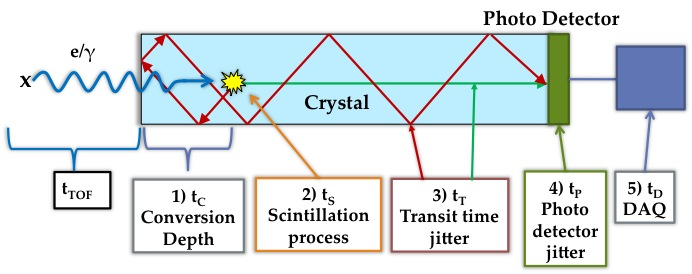
\includegraphics[width=0.85\textwidth]{figs/ScintillatorTiming} \caption{Factors
influencing the precision of the timing measurement with a monolithic, large
scintillating crystal. The incident particle impinges on the crystal face from
the left. Characteristic times of various factors are defined in the colored
boxes and in the text.}
\label{fig:ScintillatorTiming}
\end{figure}

The scintillation light produced needs to be detected. Typically this is done
with one or several photo detectors attached to the scintillator. The time $t_T$
it takes the scintillation photons to travel through the crystal may vary
substantially due to the isotropic angular distribution of the scintillation
light and the possible internal reflection of the light inside the crystal
before eventually reaching the photo detector. Finally, the photo detector and
its readout system have characteristic time constants $t_P$ and $t_D$ which will
affect the precision of the measurement as well.

In this study we focus on studying the effects of the shower development,
scintillation light emission and light propagation inside the crystal. Since the
photodetectors and readout system are shared with the experiment described
in~\cite{MCPFastCaloNIMA}, the chararacteristic times $t_P$ and $t_D$ are shared
between these two measurements. In our measurements in
Ref.~\cite{MCPFastCaloNIMA} we found the time-of-flight resolution between the
Photek 240 detectors to be $\sim 15$psec~\footnote{Here and in the following we
refer the standard deviation of the Gaussian fit as the ``resolution''}.
Assuming that the resolution of both Photek 240 is the same, one can derive the
time resolution of a Photek 240 to be $15/\sqrt{2}\approx$11 ps. The electronic
resolution of the DRS4 board was found to be $5-7$ psec. 

\begin{figure}[h] \centering
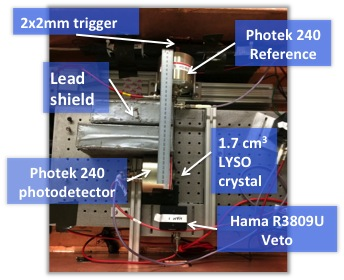
\includegraphics[width=0.5\textwidth]{figs/SetupLYSO} 
\caption{Experimental
setup for the test beam measurements. Inside a light tight box, shielded against
environmental noise, a LYSO crystal is mounted on one of the Photek 240
detectors. In all measurements the 2x2 mm$^2$ scintillator was used for
triggering. The reference Photek 240 is placed right after the trigger, and a
Hamamatsu R3809 MCP is placed behind the crystal as a Veto detector. Lead bricks
are placed upstream of the Photek 240 that reads out the crystal, to shield the detector from 
direct hits on MCP-PMT detector from beam particles.} 
\label{fig:SetupLYSO}
\end{figure}


In all results presented here which invoke the MCP based reference detector
measurement we did not unfold its contribution to the final result. In the
initial studies presented here we focus on measurements which allow to quantify
the contribution of the showering process in the crystals, the scintillation
light emission and the light propagation inside the crystal. These contributions
will dependent on the type of scintillator used, its size and its surface
properties. Future experiments will be carried out to study all these factors in
detail.

\section{Event Selection and Analysis}
To assign a time stamp for each signal
pulse, we use different procedures for the reference detector and for the one
with LYSO crystal, since their pulses have different shapes. The pulse from the
reference detector is a very sharp and symmetric around its maximum amplitude,
as shown in Figure~\ref{fig:PulseShapes}. Therefore, for the reference detector
the assignment of a time stamp is the following. We first determine the time
position of the pulse peak. A Gaussian function is fitted to the pulse maximum
using three points before the maximum of the pulse peak and four points after
the maximum. The mean value of the Gaussian fitted function was used as the time
stamp for each pulse. A time stamp for the scintillation light is assigned using
constant fraction fit on the rising edge. We perform a fit with a linear
function between the points at 20\% and 70\% of the maximum of the pulse peak,
and the time stamp is assigned as the midpoint of the fitted function. Examples of fits performed to assign a time stamp from each pulse are shown in Figure~\ref{fig:PulseFits}.

\begin{figure}[h] \centering
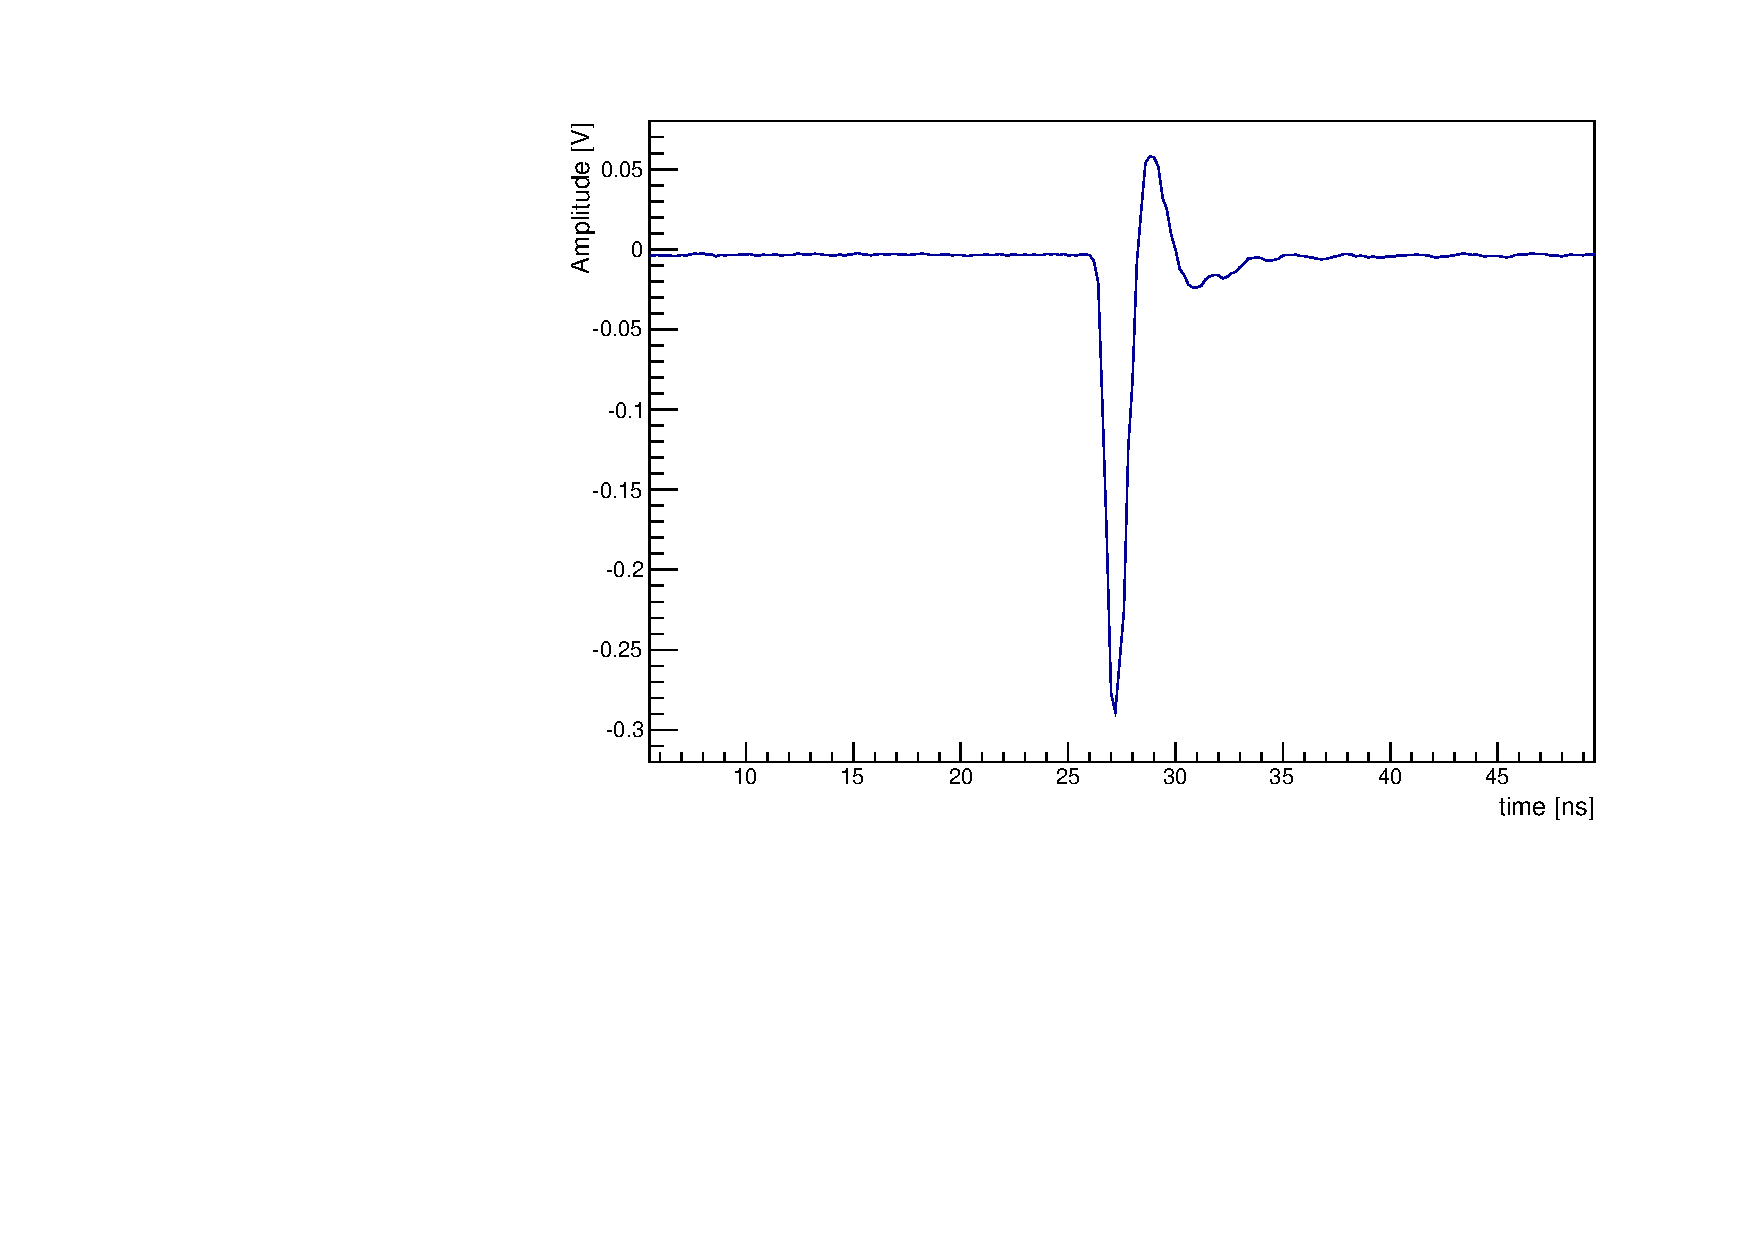
\includegraphics[width=0.45\textwidth]{figs/RefPulse} 
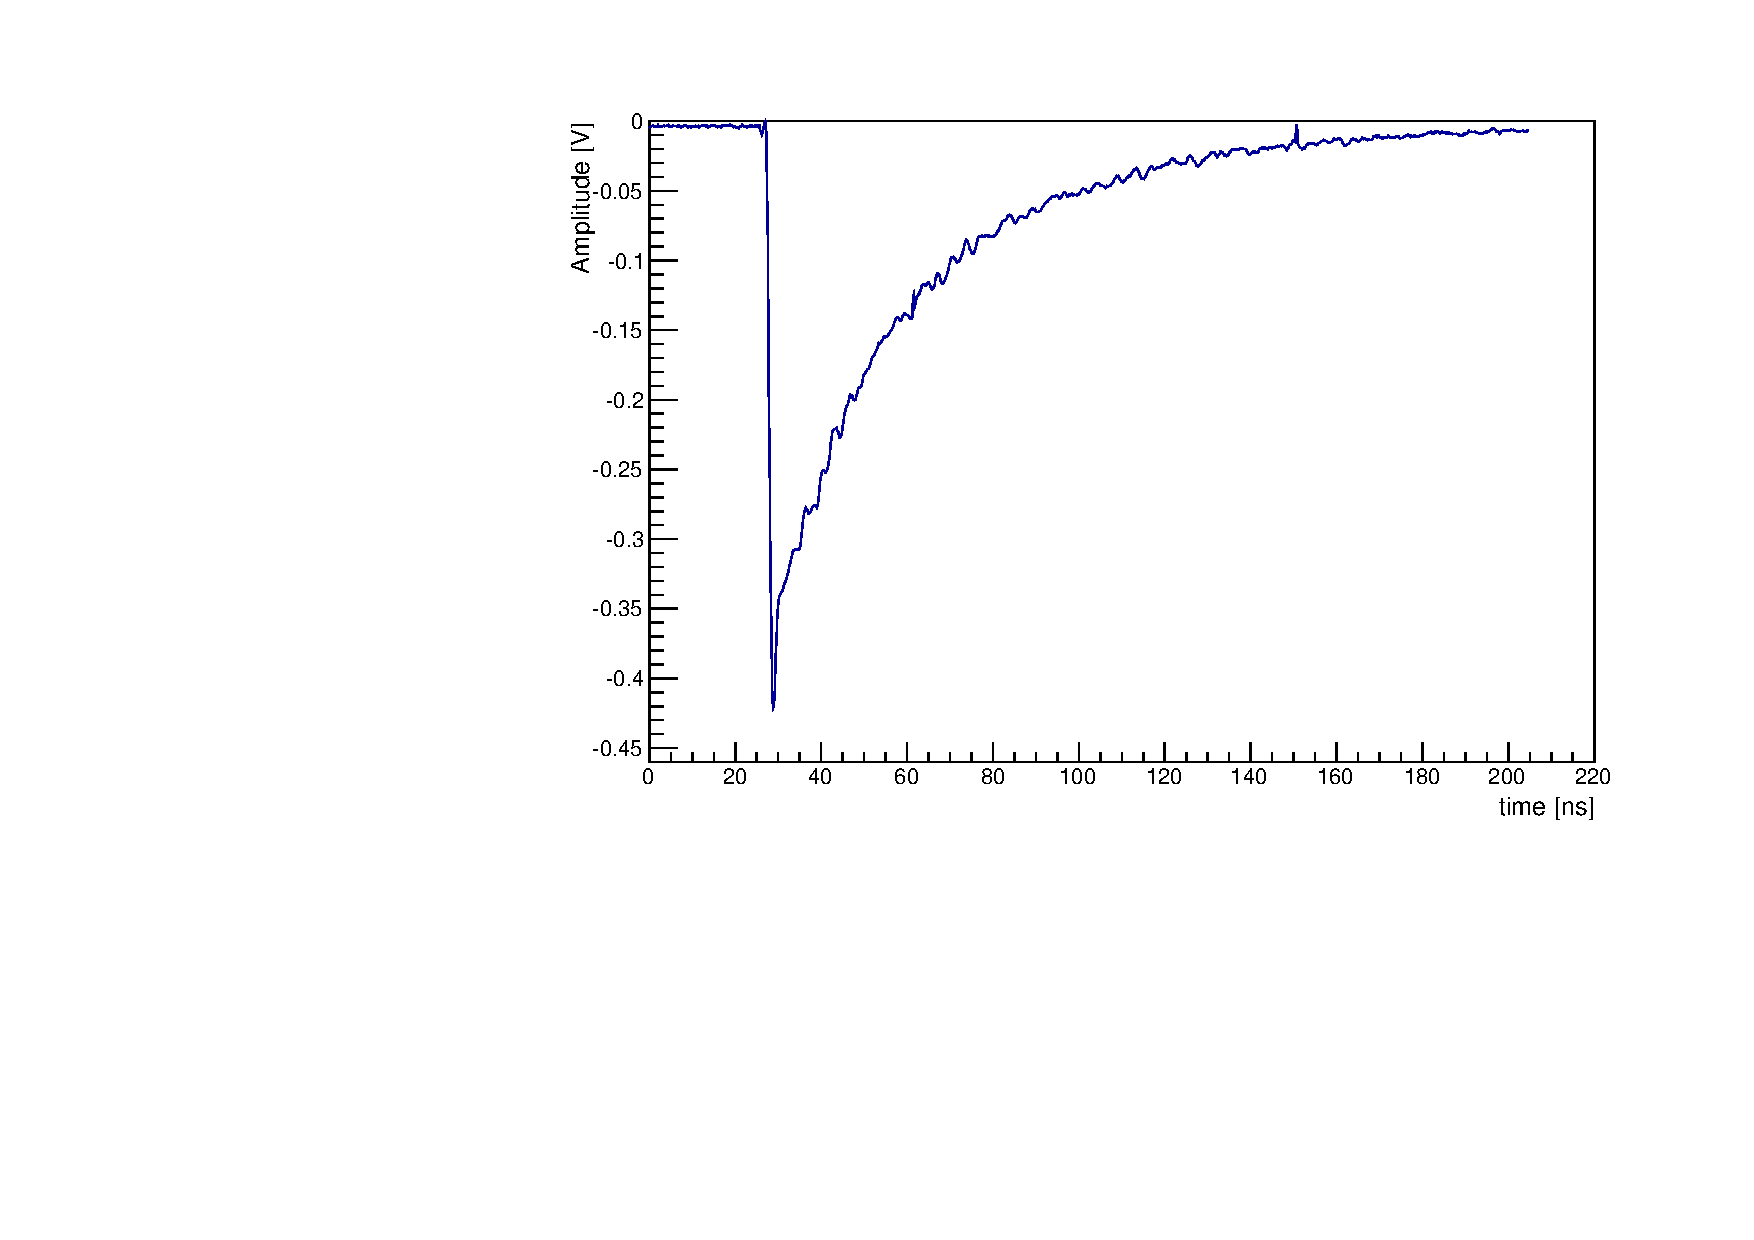
\includegraphics[width=0.45\textwidth]{figs/ScintPulse} 
\caption{Sample pulses as digitized by the DRS4 board. (Left) is a  pulse from the reference Photek 240, and (right) is a  pulse from 1.7 cm$^3$ LYSO crystal, from an 8 GeV electron run.} 
\label{fig:PulseShapes}
\end{figure}

Event selection and pulse cleaning procedure was used to eliminate abnormal
pulses in the readout. Large signals above 500 mV were also rejected because
they saturated the DRS4 inputs. Pulses with an irregular peak profile were
rejected, as well as pulses which experienced a sudden reversal of polarity that
is occasionally observed with our readout. We selected the pulses with amplitude
larger than 20 mV for future analysis. Events containing more than one pulse
within our readout window of 200 ns were not used. 

\begin{figure}[h] \centering
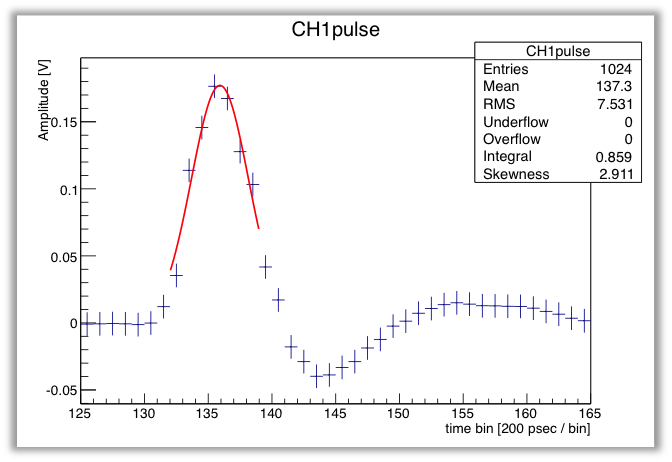
\includegraphics[width=0.45\textwidth]{figs/RefPulseFit} 
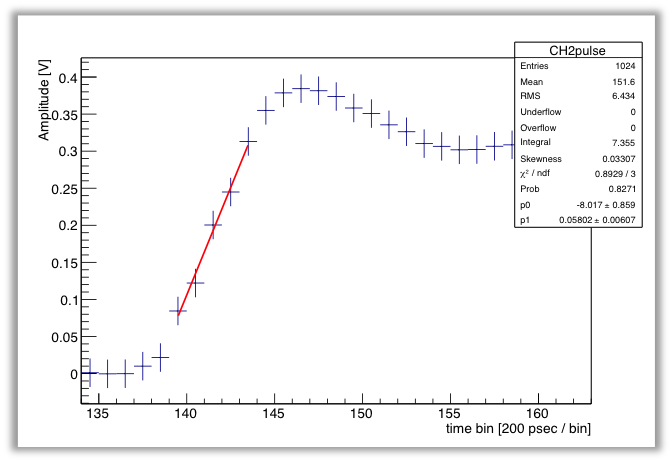
\includegraphics[width=0.45\textwidth]{figs/ScintPulseFit} 
\caption{Sample fits to assign a time stamp to the each pulse. (Left) is a  pulse from the reference Photek 240, and (right) is a  pulse from 1.7 cm$^3$ LYSO crystal, from an 8 GeV electron run.} 
\label{fig:PulseFits}
\end{figure}


\section{Time of Flight in a Crystal-based Sampling Calorimeter}

As we discussed in the introduction, this article describes studies
focused on the characterization of two of the five main aspects
driving the time of flight resolution: scintillation and 
optical transport. Stochastic processes in the scintillation
mechanism and the randomization of the optical paths for the 
scintillation light to reach the location of the photodetector 
affect both the speed of the signal formation
as well as the time jitter. We characterize the impact of
these two effects on the time of flight resolution using
two independent experimental setups which isolates the
two components. To study the effect of scintillation
we perform time of flight resolution measurements
for electron beams using a sampling calorimeter composed of a 
$(1.7\mathrm{ cm})^{3}$ LYSO cube as the active 
scintillating element behind about 4 radiation lengths of lead. 
The effect of optical transport is studied by measuring
the time of flight resolution using a shashlik 
calorimeter composed of alternating layers of tungsten
and LYSO, with scintillation light signal extracted
through wavelength shifting fibers as well as 
through direct optical coupling to the edges of a few
LYSO layers. 


\subsection{Sampling Calorimeter Setup}


In this section we report results of the
measurements of the time-of-flight (TOF) resolution performed in different
geometric setups. We studied TOF resolution extracted with crystals of various
sizes, with the goal to understand the impact of transit time jitter with
differing sizes of scintillating medium. Additionally, we report our
measurements with a LYSO/W Shashlik cell configuration, which is one of the
calorimeter designs that is being considered for CMS HL-LHC upgrades. In all the
measurements the signal of the first Photek 240 was always used as ``start''.
The signal of the ``stop'' counter was taken from the second in line MCP-PMT,
connected to the LYSO crystal. In all cases with electron beams we require that
the Cherenkov counters located upstream have a signal constant with that of an
electron. 

First we measured the TOF resolution of a 1.7 cm$^3$ LYSO crystal shown in the
setup in Figure~\ref{fig:SetupLYSO}. The TOF is measured with respect to the
reference detector. The crystal is mounted on the face of the Photek 240 through
optical grease, and is wrapped in Tyvek. To ensure that the events selected for
analysis are indeed from showering electrons, we require that all events contain
large signals in the downstream Hamamatsu R3809 detector. As it is shown in
Figure~\ref{fig:SetupLYSO}, we place lead bricks in front of the Photek 240
mounted on the LYSO crystal. This is done to ensure that the scintillation light
signal is not contaminated by the fast rising edge of the light produced in the
entry window of the MCP-PMT, thus prohibiting direct passage of beam particles
through the MCP entry window. As a cross-check, we also collected data in
dedicated runs when the Photek 240 was replaced by a XP2020 PMTs, and found that
the pulse shapes looked identical to those from Photek, indicating that the
pulse shape is dominated by the scintillation light, and not by secondary
particles from the shower. The TOF resolutions we obtained are shown in
Figure~\ref{fig:ResolSmallXtal}, and are found to be in the range of 28-30~ps
for the energy range shown. The trigger size of 2~mm will cause geometric spread
of the mean shower position, and future tests are planned to be performed with a
smaller area trigger counters.


\begin{figure}[h] 
\centering
%\includegraphics[width=0.32\textwidth]{figs/Resol8GeVele} 
%\includegraphics[width=0.32\textwidth]{figs/Resol16GeVele} 
%\includegraphics[width=0.32\textwidth]{figs/Resol32GeVele} 
%\begin{overpic}[width=0.32\textwidth,grid,tics=10]{figs/Resol16GeVele}\put (20,50) {$\gamma$}\end{overpic}
\begin{overpic}[width=0.32\textwidth]{figs/Resol8GeVele}\put (14,52) {\footnotesize$\sigma=34$~ps}\end{overpic}
\begin{overpic}[width=0.32\textwidth]{figs/Resol16GeVele}\put (14,52) {\footnotesize$\sigma=28$~ps}\end{overpic}
\begin{overpic}[width=0.32\textwidth]{figs/Resol32GeVele}\put (14,52) {\footnotesize$\sigma=28$~ps}\end{overpic}
\caption{Time of flight results for the 1.7 cm$^3$ LYSO crystal. The results show the time difference between the reference Photek 240 and the signal extracted from the Photek 240 attached to the crystal. Results are shown for 8 GeV (left), 16 GeV (center), and 32 GeV electron beam runs. Standard deviation of the Gauss fit is overlaid on each figure.}
\label{fig:ResolSmallXtal}
\end{figure}

Next we perform measurements with a smaller size LYSO crystals, which target
characterization of the timing properties that can be applied to a Shashlik
design LYSO/W sampling calorimeter which is considered for CMS HL-LHC upgrade. A
key feature of LYSO is its high light yield. This makes a sampling calorimeter
with LYSO as active medium a feasible design. Even with a sampling fraction of
around 0.1 and a readout of the LYSO plates via fibers the effective light yield
for high energy showers is still be large enough to achieve an acceptable
stochastic term in the energy resolution. The CMS collaboration at LHC is
currently studying the feasibility of a sampling calorimeter with LYSO as active
medium and tungsten as absorber. The results we presented above indicate that
the achievable time resolution for high energy particles in a large LYSO crystal
is significantly impacted by the optical transit time jitter. Shower
fluctuations and photo statistics on the other hand are less relevant for
multi-GeV electromagnetic showers. We carried out an initial
test with a LYSO plate of 14 mm x 14 mm size and 1.5 mm thickness.  As shown in Figure~\ref{fig:ShashlikTile} we
read out a single such LYSO plate by bringing one of the sides of the plate into
contact with the MCP window. We then exposed the LYSO plate to electron and
proton beams.

\begin{figure}[h] \centering
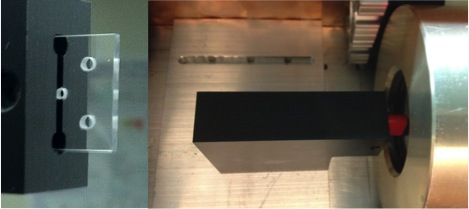
\includegraphics[width=0.45\textwidth]{figs/ShashlikTile} 
\caption{Setup for the test measurement of a single LYSO plate. The plate dimensions are 14 mm x 14 mm x 1.5 mm. It is mounted in a plastic holder which fixes the scintillator plate against the window of the MCP.} 
\label{fig:ShashlikTile}
\end{figure}

Results from the initial tests suggest that the rise time observed on the pulses
from the LYSO plate is not significantly different from the one observed on
larger LYSO crystals. We were able to extract time resolutions on the order of
50 ps with respect to the reference MCP detector, however with our initial setup it was
not possible to control the shower position on the LYSO plate very well. Also,
the signal from the MCP may have contributions from shower particles hitting the
sensor directly. Future tests with a refined setup will allow to disentangle the
contribution of the signal from direct hits and from scintillation light. 

We also tested timing characteristics of a Shashlik design cell, which consists
of LYSO tiles described above, stacked with tungsten absorber plates of
approximately 2.5 mm thickness, shown in Figure~\ref{fig:ShashlikCell}. The
fibers in the Shashlik structure were Kuraray 1.2mm non-S type, fluor (Y-11)
concentration of 300ppm. We tested two options for extracting time information
from scintillation light inside the Shashlik cell: reading out the light through
wavelength-shifting fibers; and in another setup reading out a single tile with
Hamamatsu R3809 directly mounted on it. The best TOF resolution was obtained
when reading out a single tile optically coupled to the Hamamatsu MCP-PMT, in
which case we obtained around 60 ps resolution, as shown in
Figure~\ref{fig:ShashlikCell}.

\begin{figure}[h] \centering
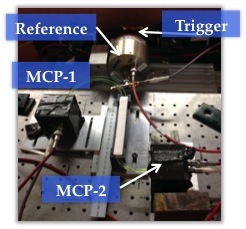
\includegraphics[width=0.32\textwidth]{figs/ShashlikSetup} 
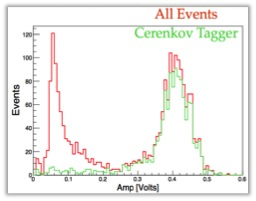
\includegraphics[width=0.32\textwidth]{figs/ShashlikEnergy} 
\begin{overpic}[width=0.32\textwidth]{figs/ShashlikResol}\put (14,72) {\footnotesize$\sigma=60$~ps}\end{overpic}
\caption{Setup for the test measurement of a LYSO/W Shashlik cell. (Left) fibers optically coupled to Hamamatsu R3809 MCP. (Center) the distribution of signal amplitudes in a sample of events collected in an 8 GeV electron run, light is collected through fibers. (Right) time difference between the reference Photek 240 and the signal extracted from  Hamamatsu R3809 attached to a single LYSO tile, 8 GeV electron beam.} 
\label{fig:ShashlikCell}
\end{figure}

\subsection{LYSO/W Shashlik Calorimeter Setup}

\section{Summary}

\end{document}  






























